\documentclass[12pt,onecolumn,draftclsnofoot]{IEEEtran}
\usepackage[a4paper,margin=1in]{geometry}
\usepackage{times,graphicx,amsmath,booktabs,cite,url}
\usepackage[ruled,linesnumbered]{algorithm2e}
% --- additions to the given preamble (packages only; no layout changes) ---
\usepackage{amssymb}
\usepackage{array}
\graphicspath{{figures/}}

\begin{document}

\title{Repository History as Retrieval Context: Evaluating Local LLMs for Design-Rationale Questions and Pull-Request Review}

\author{Group XX: Name1 (Roll No.), Name2 (Roll No.), Name3 (Roll No.), Naveen Singh/Kiran Khatter\\
School of Engineering \& Technology, BML Munjal University}

\maketitle

\begin{abstract}
Developers reviewing a change often need to know why the code is the way it is, but code assistants built on retrieval-augmented generation (RAG) usually index only the current source code, while the reasons sit in commits, issues and pull-request discussions. We present a unified platform that joins two locally hosted systems: ChangeGuard, which analyses a pull request (diff, import-graph risk, retrieved code, generated tests), and CodeOrigin, which answers ``why'' questions from code together with repository history under ten guardrails. A bridge service, a Discord bot and one dashboard connect them. We test a pre-registered hypothesis: adding history to retrieval raises correctness on history questions by at least 0.10 over code-only retrieval. On a held-out real repository (pallets/itsdangerous, 35 questions, 399 answers), history raised correctness from 0.46 to 0.78 for Llama~2 (+0.32, 95\% CI [0.07, 0.55], $p=0.022$) and from 0.42 to 0.69 for Code Llama 7B (+0.28, [0.05, 0.49]); the 3B StarCoder~2 model showed no effect. Separately, a category-wise comparison of the same three models on 27 pull-request review questions found that no single model wins every task, and that none of the 12 unit tests generated by the local models passed meaningfully, while a hosted model passed three of four once the prompt included the project's existing test file. The results show that repository history is useful evidence for capable 7B models, that the bottleneck is retrieval rather than reasoning for them, and that small models and unanswerable questions remain weak points.
\end{abstract}

\begin{IEEEkeywords}
Code review, Large language models, Mining software repositories, Pre-registered evaluation, Retrieval-augmented generation, Software maintenance
\end{IEEEkeywords}

\noindent\textbf{Overleaf Project Link:} \url{https://www.overleaf.com/project/REPLACE-WITH-YOUR-PROJECT-ID}

% =====================================================================
\section{Introduction}
% =====================================================================

Large language models (LLMs) are now part of everyday software work: they explain code, propose changes and comment on pull requests. Most of these assistants use retrieval-augmented generation (RAG) \cite{lewis2020rag,gao2023ragsurvey}, in which relevant pieces of the repository are retrieved and placed in the prompt so that the answer is grounded in the actual project. Open models such as Llama~2 \cite{touvron2023llama2} and Code Llama \cite{roziere2023codellama} can run on a single workstation, which lets a team keep its source code private while still using an assistant.

The questions developers find hardest, however, are rarely about what the code does. LaToza and Myers \cite{latoza2010hard} found that the hardest questions concern rationale: why a design was chosen, why a check exists, or what broke when a line was changed. The answers to such questions are seldom in the current code. They are in the development history: commit messages, which Tian \emph{et al.} \cite{tian2022commit} describe as the audit trail of a change, and in issues, pull requests and review comments. A reviewer who is asked to approve a change to an authentication module needs both kinds of knowledge: what the change touches, and why the touched code was written that way.

Existing tools address these needs separately. Repository-level RAG for code \cite{zhang2023repocoder} retrieves source files but not their history. Benchmarks such as SWE-bench \cite{jimenez2024swebench} use real issues and pull requests as tasks rather than as evidence for explaining design. Review assistants \cite{li2022codereviewer} generate comments from the diff, and LLM test generators \cite{schafer2024testpilot,alshahwan2024testgen} show that generated tests often fail to run. In what we found, there is no controlled comparison of \emph{history-aware} retrieval against \emph{code-only} retrieval for rationale questions, evaluated on a repository whose history was written by other people, and connected to a pull-request review workflow. Evaluations of code assistants also tend to report one blended accuracy number, which hides the fact that different models are good at different tasks. For a team choosing a model to run on its own hardware, the useful question is not which model is best overall, but which is good enough for each task at an acceptable speed, and how often it invents things.

This paper addresses two research questions:
\begin{itemize}
\item \textbf{RQ1:} Does adding repository history (commits, diffs, issues, pull requests, reviews) to retrieval improve the correctness of answers to ``why'' questions compared with retrieving current code and documentation only?
\item \textbf{RQ2:} For pull-request review tasks, which local model performs best in each task category, and are the unit tests it generates actually usable?
\end{itemize}

The contributions of this work are:
\begin{itemize}
\item A unified, locally hosted platform that joins a pull-request analyser (ChangeGuard) and a history-aware question-answering system (CodeOrigin) through a bridge service, a Discord bot with approval buttons and a single dashboard, with a shared GPU model server and live monitoring.
\item A pre-registered, four-mode evaluation design (no context, code only, code with history, and an oracle that receives the gold evidence) with a decision rule fixed before any model ran, applied to a fictional repository and to the held-out real repository pallets/itsdangerous.
\item Evidence that history raises correctness by +0.32 and +0.28 for two 7B models on the held-out repository, with retrieval diagnostics and a failure taxonomy that explain where the remaining errors come from.
\item A category-wise comparison of three local models on 27 review questions, with executed test-pass rates and an automatic detector of fabricated file and function references.
\end{itemize}

Section~II reviews related work, Section~III defines the problem, Section~IV describes the platform and method, Section~V gives the experimental setup, Section~VI reports results, Section~VII discusses them and Section~VIII concludes.

% =====================================================================
\section{Related Work}
% =====================================================================

\subsection{Retrieval-augmented generation}
RAG retrieves evidence before generating an answer \cite{lewis2020rag}; Gao \emph{et al.} \cite{gao2023ragsurvey} survey the design choices that follow, such as chunking, retrieval and grounding. Dense retrieval \cite{karpukhin2020dpr} and sentence embeddings \cite{reimers2019sbert} match text by meaning, while BM25 \cite{robertson2009bm25} matches exact terms; reciprocal rank fusion \cite{cormack2009rrf} is a simple way to combine the two rankings. Exact terms matter for repositories, where questions mention commit hashes, issue numbers and identifiers, so CodeOrigin uses the hybrid of both.

\subsection{Repository context for code models}
RepoCoder \cite{zhang2023repocoder} showed that retrieving from the whole repository improves code completion. SWE-bench \cite{jimenez2024swebench} turned real GitHub issues and pull requests from Python projects into tasks that a model must resolve. Both treat the repository's current code as the context. Tian \emph{et al.} \cite{tian2022commit} studied what makes commit messages useful and found that good messages explain both what changed and why, which is the property our work relies on. LaToza and Myers \cite{latoza2010hard} provide the motivating evidence that rationale questions are among the hardest for developers to answer.

\subsection{Models for code}
Code Llama \cite{roziere2023codellama} adapts Llama~2 \cite{touvron2023llama2} to code, StarCoder~2 \cite{lozhkov2024starcoder2} is trained on a large permissively licensed code corpus, and DeepSeek-V3 \cite{deepseek2024v3} is a much larger hosted model. Chen \emph{et al.} \cite{chen2021codex} established the practice of judging generated code by running tests, which we follow for ChangeGuard's generated tests. Model reports of this kind usually rank models on code-completion benchmarks, where the task is to write a function from its description. They say little about how a model behaves inside a retrieval pipeline, where it must read evidence it did not choose, ignore parts that do not apply and admit when the evidence is silent. A code-tuned model can therefore rank well on completion and still invent file names when asked to explain an unfamiliar repository, which is why we compare the same models per task inside our own pipeline instead of relying on published rankings.

\subsection{Review and test generation}
Bacchelli and Bird \cite{bacchelli2013review} found that reviewers mainly want to understand a change, not just find defects. CodeReviewer \cite{li2022codereviewer} pre-trains a model to write review comments. For tests, Sch\"afer \emph{et al.} \cite{schafer2024testpilot} evaluated LLM-generated unit tests at scale, and Meta's TestGen-LLM \cite{alshahwan2024testgen} keeps only generated tests that build, pass reliably and add coverage, which shows that ``the test compiles'' is not the same as ``the test is useful''.

\subsection{Reliability and evaluation}
LLMs hallucinate unsupported content \cite{ji2023hallucination}, are distracted by irrelevant context \cite{shi2023distracted}, and can be steered by instructions hidden in retrieved text \cite{greshake2023injection}. The last point matters here because commit messages and issues are written by anyone with access to the repository. For evaluation, pre-registration \cite{nosek2018prereg} protects against choosing the analysis after seeing the data, Dror \emph{et al.} \cite{dror2018significance} recommend paired significance tests for NLP comparisons, and Zheng \emph{et al.} \cite{zheng2023judge} show that LLM judges agree reasonably with humans but have biases, so they should be validated rather than trusted. Taken together, these studies suggest that extra context is not free: history adds relevant evidence, but it also adds text that can distract the model or carry injected instructions, so any gain from history has to be measured against a code-only baseline and checked on questions where history should not matter.

\subsection{Critical comparison}
Table~\ref{tab:related} compares eight works most relevant to ours. Three gaps appear. First, studies that use the repository as context use its current state, not its history, and studies that use history (issues, pull requests) use it as a task to solve rather than as evidence for explaining design. Second, most evaluations report a single accuracy figure and do not separate retrieval failure from model failure; an oracle condition, which hands the model the gold evidence, is rarely used. Third, generated tests are often counted when they compile, although \cite{alshahwan2024testgen} shows that many such tests do not pass or add nothing. \textbf{Research gap:} no published work we found compares history-aware and code-only retrieval for rationale questions under a pre-registered rule on a held-out real repository, and combines it with a per-category model comparison for pull-request review that counts only tests that actually pass.

\begin{table}[!t]
\caption{Comparison of key related work}
\label{tab:related}
\centering
\scriptsize
\setlength{\tabcolsep}{3pt}
\begin{tabular}{@{}p{0.9cm}p{1.6cm}p{1.9cm}p{1.7cm}p{1.3cm}p{2.2cm}p{2.0cm}p{1.6cm}@{}}
\toprule
Work & Problem & Method & Dataset & Metrics & Key result & Limitation & Relevance \\
\midrule
\cite{lewis2020rag} & Knowledge-intensive QA & Dense retriever + generator & Open-domain QA sets & Exact match & Retrieval improves factual answers & Wikipedia text, no code & Base RAG pattern \\
\cite{zhang2023repocoder} & Code completion & Iterative repository retrieval & RepoEval & Exact/edit match & Repository context helps completion & Current code only, no history & Code-only baseline idea \\
\cite{jimenez2024swebench} & Resolving GitHub issues & Benchmark from real issues and PRs & 2{,}294 tasks, 12 repos & Tests resolved & Models resolve few real issues & History as task, not as evidence & Real-repository setting \\
\cite{tian2022commit} & Commit message quality & Empirical study & Open-source commits & Expert labels & Good messages state what and why & No QA system & Why history holds rationale \\
\cite{li2022codereviewer} & Automating review & Pre-trained review model & Review data, 9 languages & BLEU, accuracy & Better review comments & Diff only, no history & Review-assistant baseline \\
\cite{schafer2024testpilot} & LLM unit tests & Prompted generation & npm packages & Coverage, pass rate & Useful but imperfect tests & JavaScript only & Test-pass metric \\
\cite{alshahwan2024testgen} & Improving tests in industry & Generate and filter & Meta products & Build, pass, coverage & 75\% build, 57\% pass, 25\% add coverage & Industrial, closed & Only count passing tests \\
\cite{shi2023distracted} & Irrelevant context & Controlled distractors & GSM-IC & Accuracy & Distractors lower accuracy & Arithmetic tasks & Why history can hurt \\
\bottomrule
\end{tabular}
\end{table}

% =====================================================================
\section{Background and Problem Formulation}
% =====================================================================

A repository $\mathcal{R}$ consists of its current files and its history: commits with messages and diffs, issues, pull requests, review comments and releases. Ingestion splits these into chunks, each with a type (code, documentation, commit, issue, pull request, review) and references to the objects it links to, so that an issue can lead to the pull request that fixed it and to the commits it contained. A question $q$ is answered by retrieving chunks, building a prompt within a fixed character budget and generating an answer that should cite the chunks it used. Table~\ref{tab:notation} lists the notation.

\begin{table}[!t]
\caption{Notation}
\label{tab:notation}
\centering
\small
\begin{tabular}{@{}ll@{}}
\toprule
Symbol & Meaning \\
\midrule
$\mathcal{R}$, $\mathcal{C}$ & repository; its set of chunks \\
$m \in \{\textsc{nc},\textsc{co},\textsc{ch},\textsc{or}\}$ & mode: no context, code only, code + history, oracle \\
$\mathcal{C}_m$ & chunks a mode may retrieve ($\mathcal{C}_{\textsc{co}}$: code and docs; $\mathcal{C}_{\textsc{ch}}=\mathcal{C}$) \\
$r_v(c)$, $r_b(c)$ & rank of chunk $c$ by vector similarity and by BM25 \\
$k$, $\kappa$ & retrieved chunks ($k=8$); RRF constant \\
$B$ & context budget in characters ($B=6000$) \\
$F_q$, $E_q$ & key facts and gold evidence of question $q$ \\
$s(a,q)$ & correctness of answer $a$ \\
$\Delta$ & paired gain $s_{\textsc{ch}}-s_{\textsc{co}}$ over history questions \\
$\theta_1$, $\theta_2$ & thresholds of the on-topic gate (G1) and history gate (G2) \\
\bottomrule
\end{tabular}
\end{table}

\textbf{Problem statement.} For CodeOrigin, the input is a repository $\mathcal{R}$ and a question $q$; the output is an answer $a$ with citations, or a refusal when the evidence does not support an answer. The research problem is to decide whether letting retrieval see history ($\mathcal{C}_{\textsc{ch}}$) instead of code alone ($\mathcal{C}_{\textsc{co}}$) increases $s(a,q)$ on questions whose answer lies in history, without lowering it on questions that need only the current code. For ChangeGuard, the input is a pull request (its diff and metadata) and the output is a risk level, an explanation that cites files, and on request a candidate unit test; the problem is to find which model is best for each review task and whether its tests pass.

\textbf{Assumptions and constraints.} Repositories are Git repositories, optionally hosted on GitHub so that issues and pull requests can be fetched; everything must run on one laptop with a 6\,GB GPU; the models are used without fine-tuning; prompts, budget and decoding settings are identical across modes so that only the evidence differs.

\textbf{Out of scope.} Languages other than Python for structure-aware chunking, automatic merging of pull requests (decisions are always human), private repositories requiring tokens, and large models beyond one hosted comparison run.

% =====================================================================
\section{Proposed Methodology}
% =====================================================================

\subsection{Platform architecture}
Fig.~\ref{fig:arch} shows the platform. Users reach it through a web dashboard or a Discord server. Both talk to the platform bridge, a FastAPI service that stores review decisions and an audit log in SQLite and pushes events to the dashboard as a server-sent event stream. The bridge calls two independent stacks. The ChangeGuard stack has a gateway, an orchestrator and services for Git access, code analysis, retrieval, embeddings, the LLM, test generation and persistence. The CodeOrigin stack has a gateway, an ingestion service that reads Git and the GitHub API, a hybrid retrieval service, an orchestrator that applies the guardrails, an LLM service and an evaluation service. One Ollama server on the GPU serves all models, so the two stacks do not compete for GPU memory. Prometheus and Grafana scrape CodeOrigin's metrics. We kept the stacks separate behind the bridge, instead of merging their code, so that each can be tested and evaluated on its own and so that a failure in one does not stop the other.

\begin{figure}[!t]
\centering
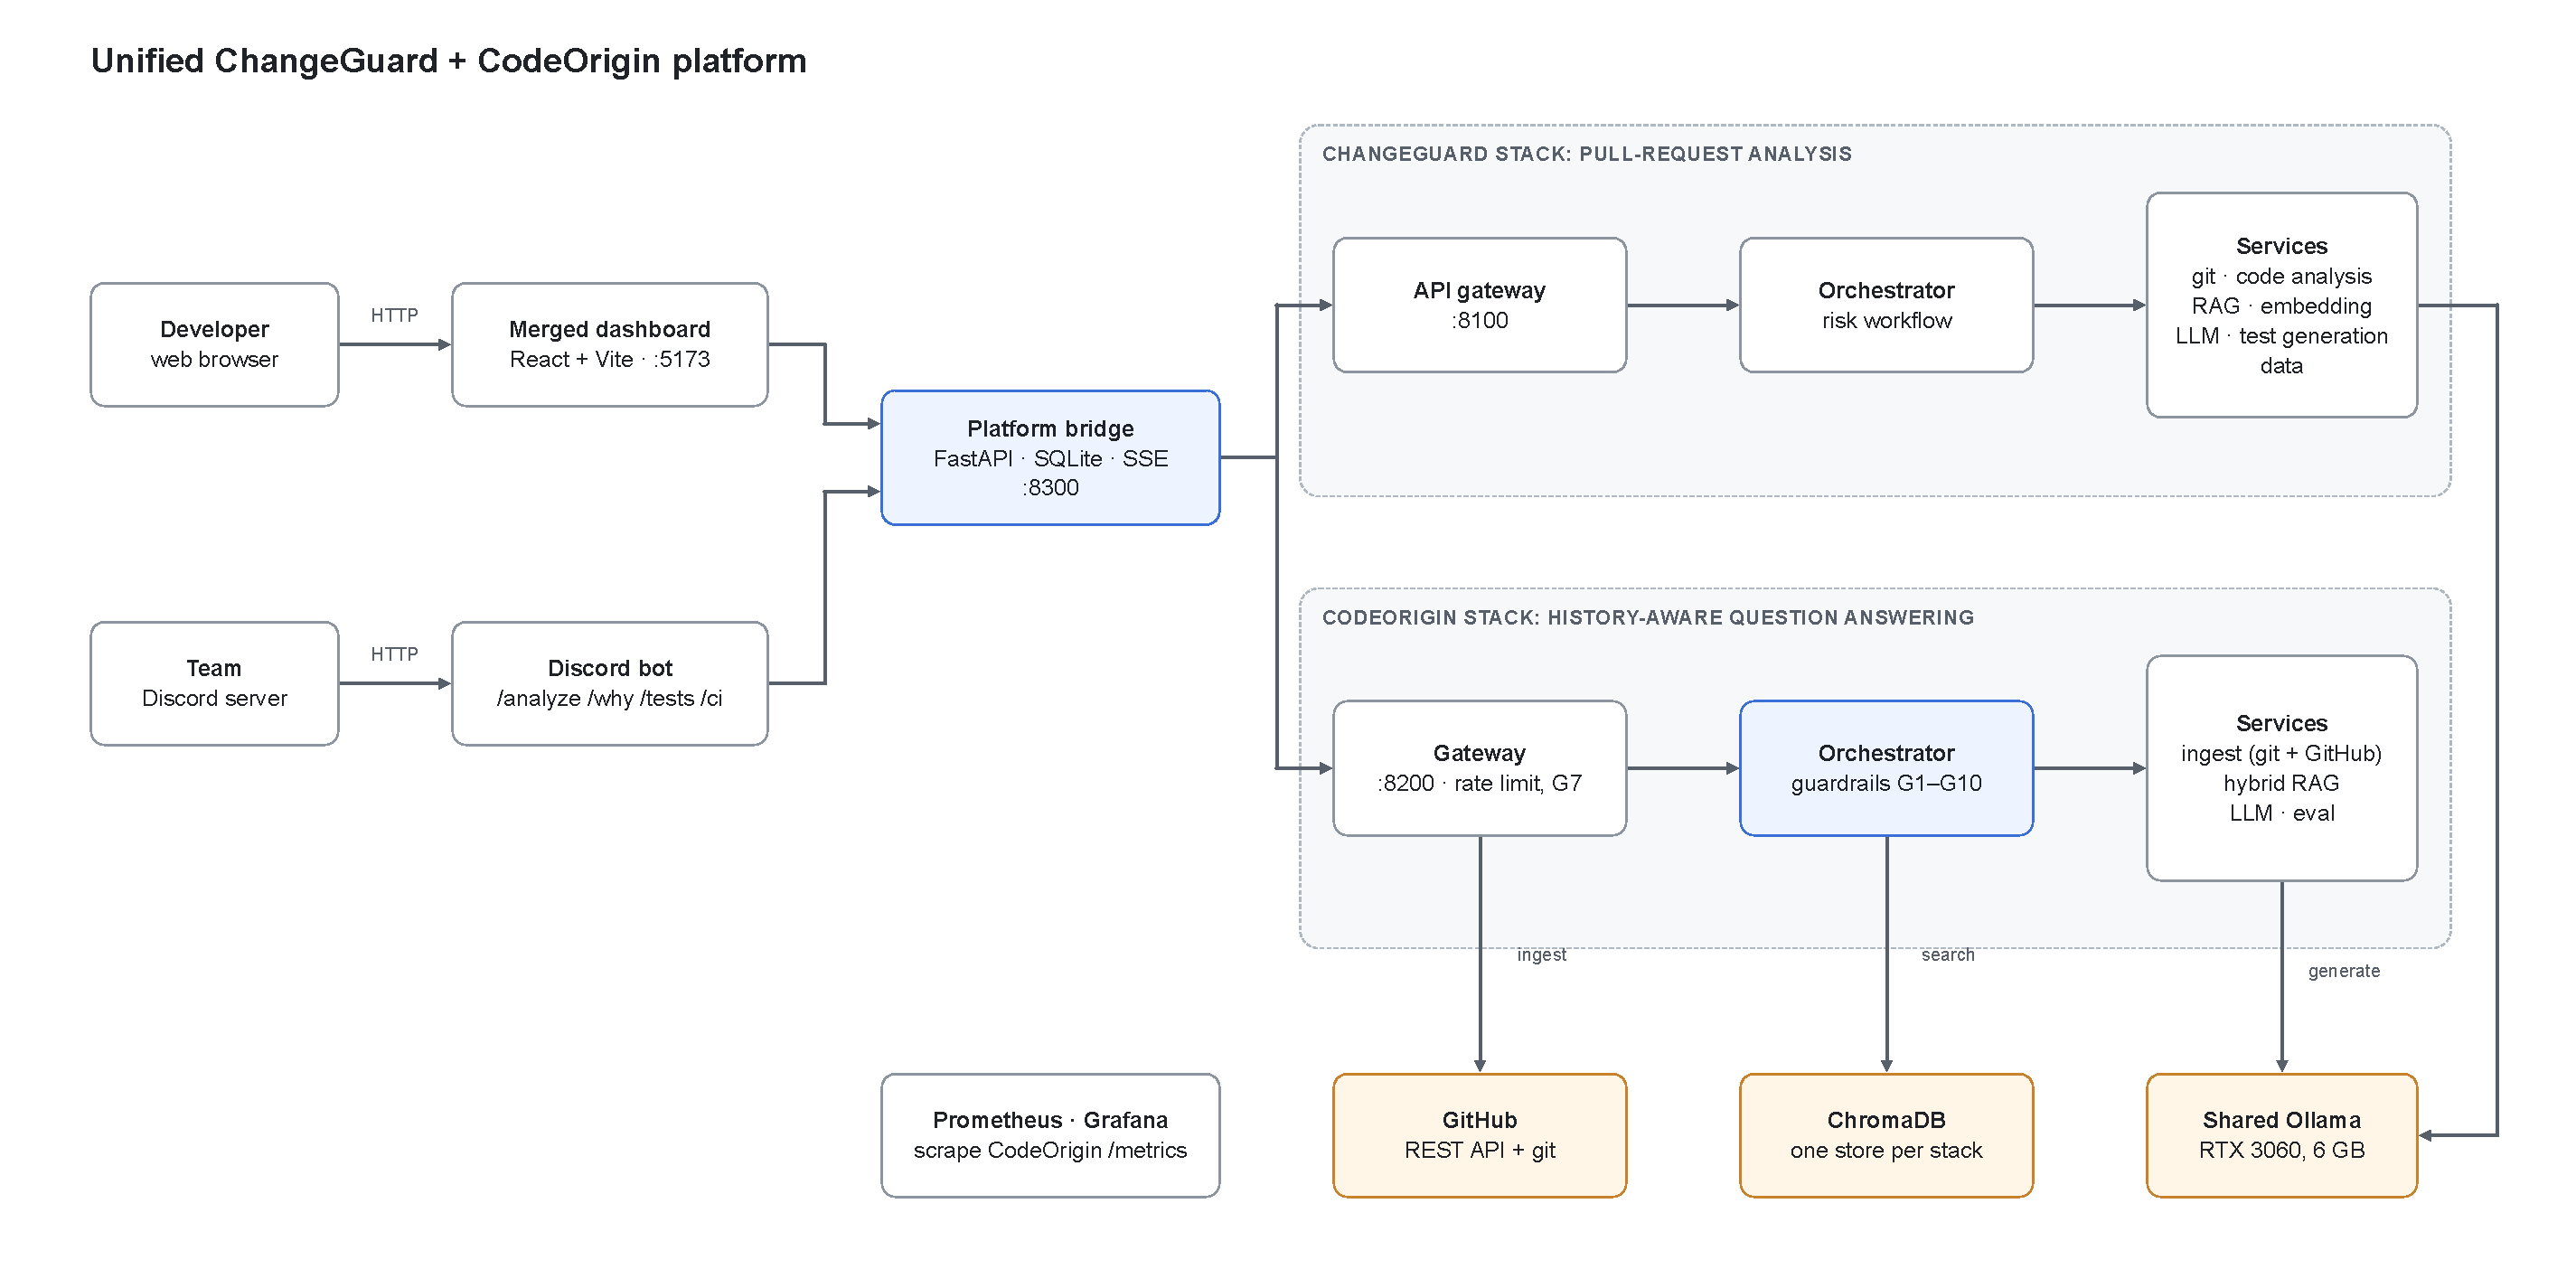
\includegraphics[width=\linewidth]{architecture.pdf}
\caption{Architecture of the unified platform. The bridge is the only component that calls both stacks; each stack keeps its own gateway, orchestrator and vector store, and both share one GPU model server.}
\label{fig:arch}
\end{figure}

\subsection{Workflow}
Fig.~\ref{fig:workflow} shows the two request paths. For a pull request (top), ChangeGuard reads the diff, computes a rule-based risk signal from a static import graph and from changed files that lack tests, retrieves the relevant code, and asks the LLM to explain the risk with file citations. Tests and a CI run are generated only when a reviewer asks for them, and the final decision is a human's Approve or Request-changes action in Discord or on the dashboard. The bridge adds CodeOrigin's history for the changed files to the review report (dashed arrow). For a ``why'' question (bottom), CodeOrigin checks the request, retrieves evidence, applies the gates, builds the context, generates an answer and checks its citations and grounding.

\begin{figure}[!t]
\centering
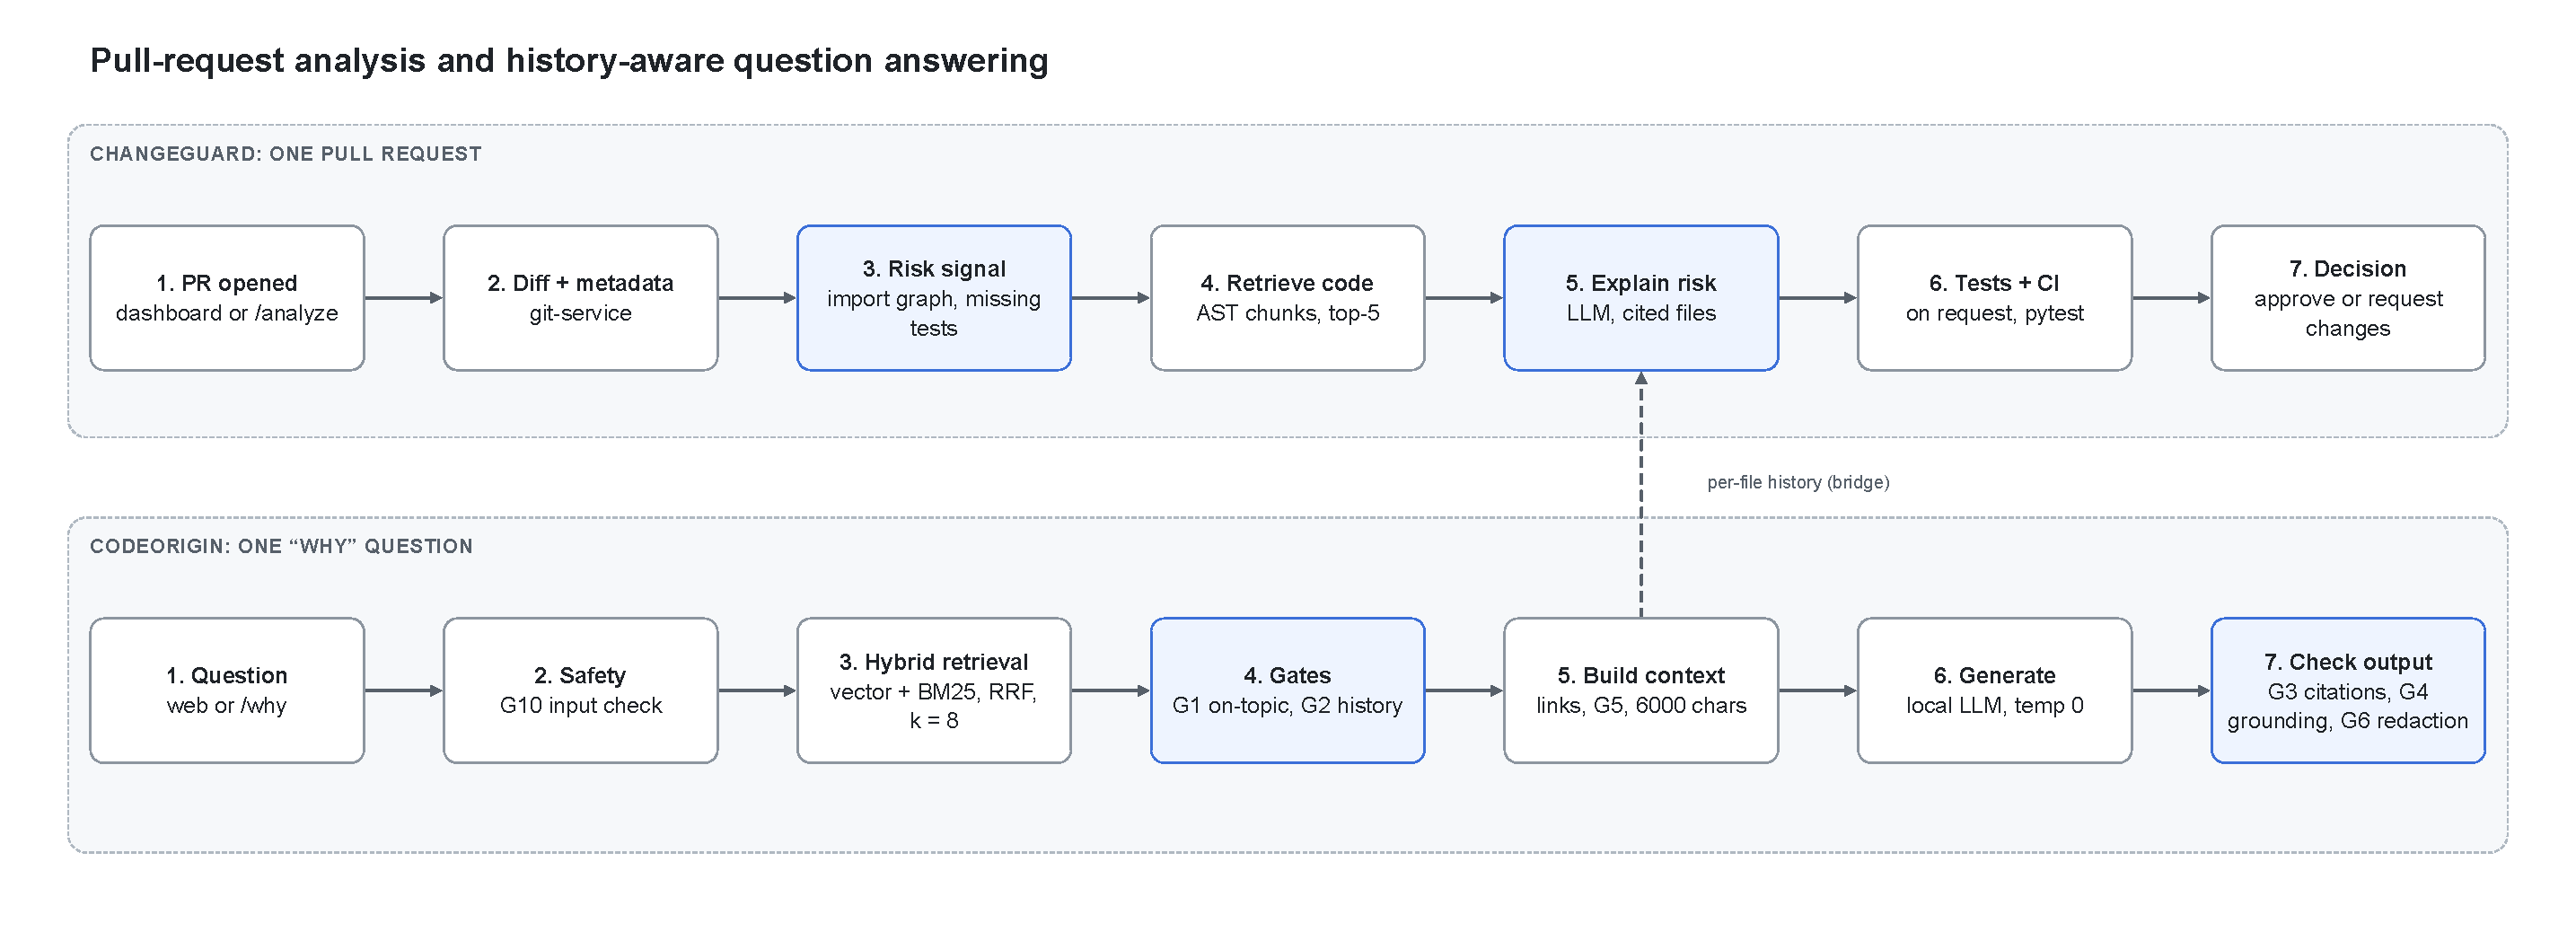
\includegraphics[width=\linewidth]{workflow.pdf}
\caption{Request workflows. Top: pull-request analysis in ChangeGuard. Bottom: one question in CodeOrigin, with the guardrails applied before and after generation. The bridge links them by adding per-file history to the review report.}
\label{fig:workflow}
\end{figure}

\subsection{History-aware retrieval}
Ingestion turns every file and history object into chunks: Python code is split at function and class boundaries with the \texttt{ast} module, Markdown at headings, and other files into line windows; issues, pull requests and reviews become chunks that keep their links. Secrets are redacted before embedding. For a question $q$, each chunk in the mode's pool $\mathcal{C}_m$ is ranked by cosine similarity of all-MiniLM-L6-v2 embeddings \cite{reimers2019sbert} and by BM25 \cite{robertson2009bm25}, and the two rankings are fused with reciprocal rank fusion \cite{cormack2009rrf}:
\begin{equation}
\mathrm{RRF}(c)=\frac{1}{\kappa+r_v(c)}+\frac{1}{\kappa+r_b(c)},\qquad c\in\mathcal{C}_m .
\label{eq:rrf}
\end{equation}
The top $k=8$ chunks are kept. We chose hybrid retrieval because questions often contain exact identifiers (``PR \#296'', a function name) that embeddings match poorly, while BM25 alone misses paraphrases. Retrieved issues and pull requests are then expanded with the commits and threads they link to, and the context is filled in rank order until the budget is reached:
\begin{equation}
X_q=\{c_1,\dots,c_j\}\ \text{with}\ \textstyle\sum_{i\le j}|c_i|\le B<\sum_{i\le j+1}|c_i| .
\label{eq:budget}
\end{equation}
The fixed budget $B=6000$ characters is the same in every mode, so a mode cannot win simply by showing the model more text.

\subsection{Guardrails}
CodeOrigin applies ten guardrails, G1--G10. Before retrieval, G10 refuses requests to reveal secrets or run commands, and G7 enforces input limits. After retrieval, G1 refuses when the best relevance is below $\theta_1$ (off-topic), and G2 answers ``the history does not say why'' when a history question finds no history chunk above $\theta_2$. G5 treats commit messages and issues as untrusted data and neutralises instruction-like text in them, because history is an obvious channel for indirect prompt injection \cite{greshake2023injection}. After generation, G3 strips citations to objects that were not retrieved, G4 flags each sentence whose words are not supported by the evidence, and G6 redacts secrets from the output. Algorithm~\ref{alg:answer} gives the complete answering procedure.

\begin{algorithm}[!t]
\caption{History-aware answering with guardrails}
\label{alg:answer}
\KwIn{question $q$, repository $\mathcal{R}$, mode $m$, budget $B$, thresholds $\theta_1,\theta_2$}
\KwOut{answer $a$ with citations, or a refusal}
\lIf{G10 or G7 rejects $q$}{\Return refusal}
\uIf{$m=\textsc{or}$}{$X \leftarrow E_q$ \tcp*{oracle: gold evidence, no retrieval}}
\uElseIf{$m=\textsc{nc}$}{$X \leftarrow \varnothing$ \tcp*{no context: no retrieval, no gates}}
\Else{
  $H \leftarrow$ top-$k$ chunks of $\mathcal{C}_m$ by $\mathrm{RRF}$ (Eq.~\ref{eq:rrf})\;
  \lIf{$\max_{c\in H}\mathrm{rel}(c) < \theta_1$}{\Return refusal (G1, off-topic)}
  \If{$q$ asks about history \textbf{and} no history chunk in $H$ has $\mathrm{rel}\ge\theta_2$}{\Return ``the history does not say'' (G2)}
  $H \leftarrow H \cup$ linked commits, issues and pull requests\;
  $X \leftarrow$ neutralise instruction-like text in $H$ (G5), then fill to budget $B$ (Eq.~\ref{eq:budget})\;
}
$a \leftarrow$ LLM(prompt$(q, X)$) at temperature 0\;
remove citations in $a$ to objects not in $X$ (G3)\;
flag sentences of $a$ with lexical support below 0.5 (G4); redact secrets (G6)\;
\Return $a$\;
\end{algorithm}

\subsection{Pull-request analysis and test generation}
ChangeGuard's code-analysis service parses the diff and scans the repository's imports to find modules that depend on the changed files and changed areas that have no tests; these form a rule-based risk signal. The retrieval service indexes the repository with structure-aware chunks (Python functions and classes; Markdown sections) and returns the top five. The LLM service assigns a model per task, so that a code-tuned model can be used for test generation and the default model for risk explanations. Generated tests are written to a temporary copy of the repository and executed with \texttt{pytest}, because a test that only compiles says little about its value \cite{alshahwan2024testgen}. Tests are candidates only and are never merged automatically.

\subsection{Scoring}
An answer is scored against the question's key facts $F_q$, each with alternative phrasings:
\begin{equation}
s(a,q)=\begin{cases}\dfrac{|\{f\in F_q : f \text{ occurs in } a\}|}{|F_q|} & \text{if } q \text{ should be answered},\\[6pt] \mathbf{1}[a \text{ is a refusal or abstention}] & \text{if } q \text{ should be refused.}\end{cases}
\label{eq:score}
\end{equation}
The history gain is the mean paired difference over the $n$ history questions,
\begin{equation}
\Delta=\frac{1}{n}\sum_{i=1}^{n}\big(s_{\textsc{ch},i}-s_{\textsc{co},i}\big),
\label{eq:delta}
\end{equation}
with a 95\% bootstrap confidence interval (2000 resamples) and a two-sided sign-flip permutation test, as recommended for paired NLP comparisons \cite{dror2018significance}, and the effect size $d_z=\bar{\Delta}/\mathrm{sd}(\Delta_i)$. We chose key-fact matching over an LLM judge as the primary score because it is deterministic and can be recomputed from the stored answers; LLM judges are used only to validate it. The answer is counted as hallucinated when at least half of its sentences fail the G4 support check.

% =====================================================================
\section{Experimental Setup}
% =====================================================================

\textbf{Datasets.} Table~\ref{tab:data} summarises the three evaluation sets. The CodeOrigin sets have question categories for history (design rationale, bug origin, change attribution, issue linkage, evolution), a control category (current state, where history should not be needed) and guardrail behaviour (unanswerable, off-topic, adversarial). The held-out set was drafted from real issue and pull-request threads of pallets/itsdangerous, checked by a script that every gold reference exists and every key fact occurs in the cited text, and committed before any result was seen. Guardrail thresholds were calibrated on the demo set's development split only.

\begin{table}[!t]
\caption{Evaluation datasets}
\label{tab:data}
\centering
\small
\begin{tabular}{@{}p{3.2cm}p{4.6cm}p{2.3cm}p{3.6cm}@{}}
\toprule
Set & Repository & Questions & Use \\
\midrule
CodeOrigin demo & Ledgerly (fictional, 13 commits) & 43 (23 dev) & dev run 5, calibration \\
CodeOrigin held-out & pallets/itsdangerous: 677 commits, 125 issues, 311 PRs, 7 releases & 35 (24 history, 4 control, 7 guardrail) & runs 8 and 10, headline \\
ChangeGuard & demo repository (auth module, 3 commits) & 27 in 8 categories & model comparison \\
\bottomrule
\end{tabular}
\end{table}

\textbf{Baselines.} For RQ1 the baseline is the \textsc{co} mode, which runs the same pipeline but retrieves only code and documentation; it represents how most code assistants work. The \textsc{nc} mode shows what a model guesses unaided, and the \textsc{or} mode, which receives the gold evidence, separates retrieval failure from model failure. For RQ2 the three models are compared with each other on identical retrieved context, and fixed-size chunking (800 characters, 150 overlap) and unfiltered retrieval are the baselines for the retrieval settings.

\textbf{Metrics.} Correctness (Eq.~\ref{eq:score}) measures whether the answer states the right facts; evidence recall and precision measure whether the gold evidence reached the prompt and how much of the prompt it was; the hallucination rate (G4) measures unsupported content; citation validity is the share of cited references that were really retrieved; latency and tokens measure cost. For ChangeGuard, precision@5 is the share of expected files among the top five chunks; correctness, relevance and hallucination were graded by hand per answer against a gold answer; fabricated references are file paths, line ranges and function names cited in an answer that do not exist in the repository; and test pass rate counts generated tests that run and pass, with ``meaningful'' passes excluding tests that would pass regardless of the code under test.

\textbf{Decision rule.} Fixed before any model ran: history is \emph{useful} if $\Delta\ge0.10$ on the history categories, its 95\% interval excludes 0, and the control category loses at most 0.05; otherwise the result is \emph{inconclusive} or \emph{does not help} \cite{nosek2018prereg}. Results are reported per category, never as one blended score.

\textbf{Tools and settings.} All services are Python 3 with FastAPI, ChromaDB 1.0.0 and sentence-transformers, deployed with Docker Compose; the dashboard uses React, Vite and Tailwind. Models run on Ollama on a laptop with an NVIDIA RTX 3060 (6\,GB). Table~\ref{tab:params} lists every setting.

\begin{table}[!t]
\caption{Experimental parameters}
\label{tab:params}
\centering
\small
\begin{tabular}{@{}p{3.4cm}p{4.0cm}p{7.6cm}@{}}
\toprule
Component & Parameter & Value \\
\midrule
Models (Ollama tag, digest) & candidates & llama2 (78e26419b446), codellama:7b (8fdf8f752f6e), starcoder2:3b (9f4ae0aff61e) \\
Hosted comparison & model & DeepSeek API (deepseek-flash), run 10, held-out set only \\
Decoding & temperature, seed, max answer & 0, 42, 300 tokens \\
Ollama & context, KV cache, attention & 3072 tokens, q8\_0, flash attention \\
CodeOrigin retrieval & embedder, $k$, fusion & all-MiniLM-L6-v2, 8, RRF of vector and BM25 ($\kappa=60$) \\
CodeOrigin context & budget $B$ & 6000 characters, identical in all modes \\
Guardrails & $\theta_1$, $\theta_2$, G4 support & 0.36, 0.44, 0.50 (calibrated on dev split) \\
Statistics & bootstrap, permutation, seed & 2000 resamples, sign-flip (exact for $n\le12$), 0 \\
ChangeGuard retrieval & chunking, top-$k$ & structure-aware (AST / headings), 5 \\
ChangeGuard tests & execution & pytest in a temporary copy of the demo repository \\
Runs & repetitions & one run per configuration at temperature 0 \\
\bottomrule
\end{tabular}
\end{table}

\textbf{Runs and variance.} Each configuration was run once at temperature 0 with a fixed seed. Run-to-run variation was therefore not measured; instead, every reported mean carries a 95\% bootstrap interval over questions, which shows how much a result depends on the particular question sample. Run 8 produced 399 answers with no errors; run 5 produced 255; the hosted run 10 produced 133 in 238 seconds.

% =====================================================================
\section{Results and Analysis}
% =====================================================================

\subsection{RQ1: Does repository history help?}
Table~\ref{tab:heldout} gives the headline result on the held-out repository and Fig.~\ref{fig:modes} shows the same means with their intervals. For both 7B models, adding history raised correctness on the 24 history questions by about 0.3: from 0.46 to 0.78 for llama2 and from 0.42 to 0.69 for codellama:7b. Both intervals exclude zero and both models lose nothing on the four control questions by the automatic score, so both satisfy the pre-registered rule. starcoder2:3b gained nothing ($-0.02$), and the hosted DeepSeek model gained the most (+0.75). Against the no-context mode the gain is larger still (+0.57 and +0.55, both $p<0.001$), which shows how little the models know about this repository by themselves.

\begin{table}[!t]
\caption{Held-out repository: correctness on 24 history questions by mode, and the pre-registered test of code + history against code only (best non-oracle mode in bold)}
\label{tab:heldout}
\centering
\scriptsize
\setlength{\tabcolsep}{3.5pt}
\begin{tabular}{@{}lccccccccc@{}}
\toprule
Model & No context & Code only & Code + history & Oracle & $\Delta$ [95\% CI] & $p$ & $d_z$ & Verdict \\
\midrule
llama2 & 0.21 & 0.46 & \textbf{0.78} & 0.79 & +0.32 [+0.07, +0.55] & 0.022 & 0.52 & useful \\
codellama:7b & 0.15 & 0.42 & \textbf{0.69} & 0.83 & +0.28 [+0.05, +0.49] & 0.033 & 0.48 & useful \\
starcoder2:3b & 0.08 & \textbf{0.21} & 0.19 & 0.20 & $-$0.02 [$-$0.21, +0.17] & 1.000 & $-$0.04 & inconclusive \\
deepseek (hosted)$^{\dagger}$ & 0.06 & 0.10 & \textbf{0.85} & 0.98 & +0.75 [+0.54, +0.92] & $<$0.001 & 1.61 & useful \\

\bottomrule
\end{tabular}\\[2pt]
\parbox{\linewidth}{\footnotesize $^{\dagger}$Run 10: per-mode means are question-weighted from stored category means; interval and $d_z$ from the run report.}
\end{table}

\begin{figure}[!t]
\centering
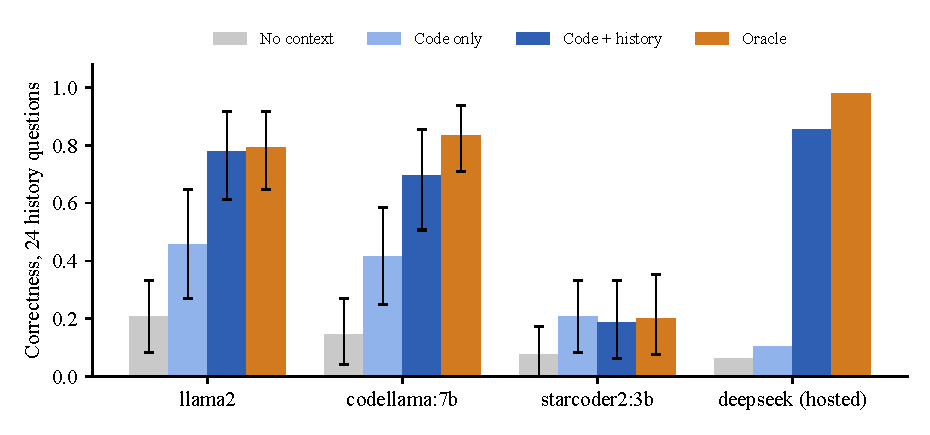
\includegraphics[width=0.95\linewidth]{fig_heldout_modes.pdf}
\caption{Correctness on the 24 held-out history questions for each model and mode. Error bars are 95\% bootstrap intervals (the hosted run stored only means).}
\label{fig:modes}
\end{figure}

The oracle column explains the mechanism. When llama2 is handed the gold evidence, it scores 0.79, almost the same as with history retrieval (0.78), so for llama2 the gain comes from finding the evidence, not from reasoning better. Table~\ref{tab:retrieval} confirms this: code-only retrieval found 14\% of the gold evidence, history retrieval 70\%. For codellama:7b the oracle still adds 0.14, so part of its remaining error is retrieval. For starcoder2:3b the oracle adds nothing (0.20): this 3B completion model does not use evidence well even when it is given the answer.

\begin{table}[!t]
\caption{Retrieval quality per mode (held-out run; identical for all models)}
\label{tab:retrieval}
\centering
\small
\begin{tabular}{@{}lcc@{}}
\toprule
Mode & Evidence recall & Evidence precision \\
\midrule
code only & 0.14 & 0.05 \\
code history & 0.70 & 0.25 \\
oracle & 1.00 & 1.00 \\
\bottomrule

\bottomrule
\end{tabular}
\end{table}

Fig.~\ref{fig:effect} places the held-out result next to the fictional demo repository. On the demo repository the gain was larger (+0.42 for both 7B models) because history and questions were written together and retrieval found all gold evidence; there, codellama's interval touched zero and its verdict was inconclusive. On the real repository the gain is smaller but both 7B intervals exclude zero, which is the stronger test because nobody on the team wrote that history.

\begin{figure}[!t]
\centering
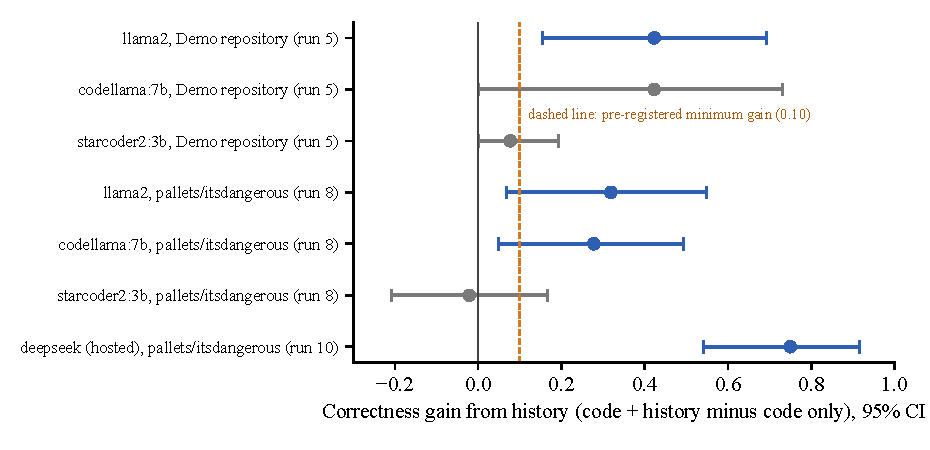
\includegraphics[width=0.95\linewidth]{fig_effect.pdf}
\caption{History gain $\Delta$ (Eq.~\ref{eq:delta}) with 95\% intervals for each model and run. Blue: interval excludes zero. The dashed line is the pre-registered minimum of 0.10.}
\label{fig:effect}
\end{figure}

\textbf{Answer quality and failures.} Table~\ref{tab:quality} reports quality and cost in the code + history mode. llama2 and codellama:7b answer about three quarters of the answerable questions correctly; codellama hallucinates less (22\% against 31\%) but is twice as slow at the median (16.1\,s against 8.3\,s). starcoder2:3b is the fastest but hallucinates in 59\% of answers, so its speed has no practical value. The failure counts show different weaknesses: llama2's few errors are mostly retrieval misses, codellama more often ignores evidence it was given, and starcoder2 mostly hallucinates. One clear negative result concerns refusals: the three unanswerable held-out questions mention the library by name, so they passed the relevance gates calibrated on the demo repository, and codellama and starcoder2 invented answers to all three. Gate G2 therefore did not transfer to a real repository.

\begin{table}[!t]
\caption{Quality, cost and failures in the code + history mode (held-out run, 35 questions)}
\label{tab:quality}
\centering
\scriptsize
\setlength{\tabcolsep}{3.5pt}
\begin{tabular}{@{}lccccccccc@{}}
\toprule
Model & Correct & Halluc. & Unsupported & Citation & Median & Retrieval & Ignored & Hallu- & Under- \\
 & (answerable) & rate & ratio & validity & latency (s) & miss & evidence & cinated & refused \\
\midrule
llama2 & 0.77 & 31\% & 0.27 & 1.00 & 8.3 & 3 & 1 & 1 & 0 \\
codellama:7b & 0.74 & 22\% & 0.26 & 0.93 & 16.1 & 2 & 3 & 1 & 4 \\
starcoder2:3b & 0.20 & 59\% & 0.37 & 0.89 & 1.4 & 6 & 5 & 10 & 4 \\
\bottomrule

\bottomrule
\end{tabular}
\end{table}

\subsection{RQ2: Which model for which review task?}
Table~\ref{tab:cg} and Fig.~\ref{fig:cg} report the ChangeGuard comparison. Retrieval was the same for all models and reached a mean precision@5 of 0.88; it was weakest for dependency questions (0.33), whose answer depends on files that import the changed one. By hand grading, codellama:7b had the best correctness in six categories (tied in one), while llama2 was best in the two categories answered from prose: bug analysis (0.67) and documentation questions (0.78). starcoder2:3b won none. The automatic key-fact score, shown for comparison, agrees on the overall ranking (0.55, 0.54 and 0.36) but not always per category; for dependency questions it credits llama2 with 0.78 while the hand grade is 0.20. The key-fact score only counts the files and identifiers an answer names, which llama2 did name, whereas the hand grade also penalised the unsupported claims it made about them. This disagreement is why hand grading was kept as the primary measure for this set.

\begin{table}[!t]
\caption{ChangeGuard: retrieval precision@5, hand-graded correctness and automatic key-fact score per category (best hand grade in bold; L = llama2, C = codellama:7b, S = starcoder2:3b)}
\label{tab:cg}
\centering
\scriptsize
\setlength{\tabcolsep}{4pt}
\begin{tabular}{@{}lccccccccc@{}}
\toprule
& & & \multicolumn{3}{c}{Hand grade} & \multicolumn{3}{c}{Key-fact score} \\
\cmidrule(lr){4-6}\cmidrule(lr){7-9}
Category & $n$ & P@5 & L & C & S & L & C & S \\
\midrule
Code explanation & 3 & 1.00 & \textbf{0.67} & \textbf{0.67} & 0.17 & 0.50 & 0.42 & 0.41 \\
Code retrieval & 5 & 0.90 & 0.70 & \textbf{0.75} & 0.30 & 0.71 & 0.84 & 0.51 \\
Dependency understanding & 3 & 0.33 & 0.20 & \textbf{0.45} & 0.03 & 0.78 & 0.67 & 0.28 \\
Bug analysis & 3 & 1.00 & \textbf{0.67} & 0.55 & 0.07 & 0.50 & 0.50 & 0.39 \\
RAG / documentation & 3 & 1.00 & \textbf{0.78} & 0.62 & 0.32 & 0.56 & 0.44 & 0.56 \\
Code generation & 4 & 1.00 & 0.16 & \textbf{0.28} & 0.04 & 0/4 pass & 0/4 pass & 0/4 pass \\
Refactoring & 3 & 1.00 & 0.17 & \textbf{0.32} & 0.00 & 0.13 & 0.13 & 0.13 \\
Repository-level & 3 & 0.72 & 0.27 & \textbf{0.32} & 0.00 & 0.53 & 0.61 & 0.10 \\
\bottomrule

\bottomrule
\end{tabular}
\end{table}

\begin{figure}[!t]
\centering
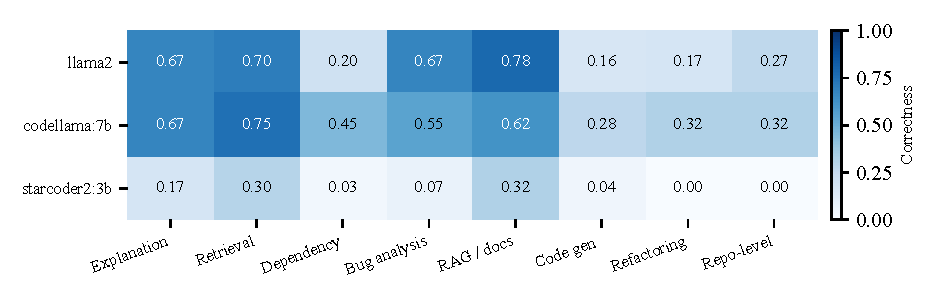
\includegraphics[width=0.95\linewidth]{fig_changeguard.pdf}
\caption{Hand-graded correctness of the three local models in each ChangeGuard task category. No model is best everywhere.}
\label{fig:cg}
\end{figure}

Table~\ref{tab:cgcost} turns to reliability and cost. The fabricated-reference detector found none of llama2's 80 cited files and functions to be invented, 2 of codellama's 82, but 11 of starcoder2's 60, affecting a quarter of its answers. The 7B models took about 50\,s per answer at the median on this hardware, against 21\,s for starcoder2. For code generation, none of the 12 stored replies passed as saved, because the replies mixed prose and code. After extracting the code, one codellama test passed, but it was vacuous: it accepted any exception and passed a string where a request object was expected. Meaningful passes therefore remained 0 of 12. Fig.~\ref{fig:cost} summarises the trade-off for both systems: the fastest model is also the least reliable.

\begin{table}[!t]
\caption{ChangeGuard reliability and cost: fabricated references, latency, throughput, container resources and generated-test outcomes (4 tasks per model)}
\label{tab:cgcost}
\centering
\scriptsize
\setlength{\tabcolsep}{3pt}
\begin{tabular}{@{}lcccccccccc@{}}
\toprule
Model & Fabricated & Answers & Median & p95 & Tokens/s & CPU & Memory & Tests pass & Pass after & Meaningful \\
 & refs & affected & latency (s) & latency (s) & & & (GiB) & (raw) & extraction & pass \\
\midrule
llama2 & 0/80 & 0\% & 47.3 & 116.1 & 4.1 & 41\% & 2.14 & 0/4 & 0/4 & 0/4 \\
codellama:7b & 2/82 & 5\% & 49.9 & 92.9 & 3.5 & 29\% & 2.26 & 0/4 & 1/4 & 0/4 \\
starcoder2:3b & 11/60 & 25\% & 20.8 & 58.0 & 14.9 & 25\% & 0.69 & 0/4 & 0/4 & 0/4 \\

\bottomrule
\end{tabular}
\end{table}

\begin{figure}[!t]
\centering
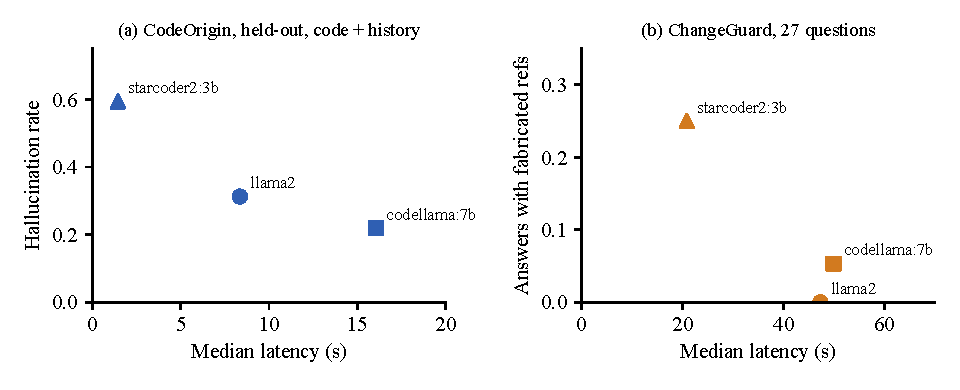
\includegraphics[width=0.95\linewidth]{fig_cost.pdf}
\caption{Reliability against speed. (a) CodeOrigin hallucination rate and median latency in the code + history mode. (b) ChangeGuard share of answers with fabricated references and median latency. In both systems the 3B model is fastest and least reliable.}
\label{fig:cost}
\end{figure}

\subsection{Ablation studies}
Table~\ref{tab:ablation} changes one component at a time. For CodeOrigin, removing history is the main experiment; removing all retrieval roughly doubles the loss; replacing retrieval with the gold evidence adds little for llama2 and starcoder2 but 0.14 for codellama; and the conclusion survives a different scorer (a DeepSeek judge gives +0.35 and +0.35) and the removal of two questions that an independent review found weak. For ChangeGuard, structure-aware chunking halved the context sent to the model (350 against 722 characters) at a small cost in precision@5 (0.90 against 1.00); restricting retrieval to source files lowered precision@5 from 0.90 to 0.60, because two questions are answered by documentation and tests; and adding the repository's existing test file to the generation prompt raised meaningful passes of the hosted model from 0 of 4 to 3 of 4. The last result locates the code-generation failure in the prompt rather than in the model: without an example, every model invented its own test doubles instead of using the project's \texttt{FakeRequest} helper.

\begin{table}[!t]
\caption{Ablations: one component changed at a time}
\label{tab:ablation}
\centering
\scriptsize
\setlength{\tabcolsep}{3pt}
\begin{tabular}{@{}p{3.6cm}p{4.4cm}p{6.6cm}@{}}
\toprule
Component & Change & Effect \\
\midrule
\multicolumn{3}{@{}l}{\emph{CodeOrigin (history gain on 24 held-out history questions; llama2 / codellama / starcoder2)}} \\
Remove history from retrieval & code only $\rightarrow$ code + history & +0.32 / +0.28 / $-$0.02 \\
Remove all retrieval & no context $\rightarrow$ code + history & +0.57 / +0.55 / +0.11 \\
Replace retrieval with gold evidence & code + history $\rightarrow$ oracle & +0.01 / +0.14 / +0.01 \\
Change repository & held-out $\rightarrow$ fictional demo (run 5) & +0.42 / +0.42 / +0.08 \\
Change the scorer & key facts $\rightarrow$ DeepSeek judge & +0.35 / +0.35 / +0.06 \\
Drop 2 weak questions & 24 $\rightarrow$ 22 questions & +0.33 / +0.27 / $-$0.02 \\
\midrule
\multicolumn{3}{@{}l}{\emph{ChangeGuard (5 retrieval questions; 4 test-generation tasks)}} \\
Chunking & fixed 800 chars $\rightarrow$ AST/structure & P@5 1.00 $\rightarrow$ 0.90; context 722 $\rightarrow$ 350 chars \\
Metadata filter & all files $\rightarrow$ source code only & P@5 0.90 $\rightarrow$ 0.60 \\
Test prompt context (DeepSeek) & no example test $\rightarrow$ retrieved test file & meaningful passes 0/4 $\rightarrow$ 3/4 \\
Code extraction before pytest & raw reply $\rightarrow$ extracted code & local passes 0/12 $\rightarrow$ 1/12 (meaningful 0/12) \\

\bottomrule
\end{tabular}
\end{table}

\subsection{Validity of the automatic score}
Because key-fact matching can miss paraphrases and reward long answers, it was compared with independent graders, all blind to model and mode. On all 399 held-out answers, a DeepSeek judge agreed with it at quadratic-weighted $\kappa=0.75$ (75\% exact agreement); on a sample of 36 answers, GPT agreed at $\kappa=0.94$ and Gemini at $\kappa=0.69$, about as well as the judges agreed with one another (0.80--0.86). The project author's hand check of 18 factual rows agreed 18 of 18. Where the score and the judge differed, the score was mostly too generous: 42 of its 143 full-credit answers were rated only partly correct, typically a right fact with an invented extra claim. The judge also disagreed on the control category, where it rated history as harmful ($-0.25$ for llama2, interval including zero), so we do not claim that history causes no loss on code-only questions.

% =====================================================================
\section{Discussion}
% =====================================================================

The results support a practical conclusion: for a 7B model on a laptop, the most effective way to answer ``why'' questions is to give it the repository's history, not a bigger model or a better prompt. The oracle comparison shows that llama2 already reasons well enough once it sees the right commit or issue; what it lacks is access. The same pattern appears in ChangeGuard's test generation, where including the project's existing test file in the prompt took the hosted model from no useful tests to three of four. In both systems the largest gains came from what was put in front of the model.

The small model behaved differently. starcoder2:3b neither benefited from history nor from the gold evidence, hallucinated in most answers and invented a quarter of its file references. Its speed is real, but a review assistant whose next answer may be unrelated code is worse than a slower, consistent one. The per-category results also show that ``the best model'' is not a single answer: codellama:7b led on code structure and llama2 on prose questions, which matches how each model was trained and supports assigning models per task, as ChangeGuard's LLM service does.

\textbf{Limitations.} The samples are small: 24 history questions and only 4 control questions on the held-out repository, and 3--5 questions per ChangeGuard category, so the intervals are wide. Each configuration was run once at temperature 0, so run-to-run variance was not measured. ChangeGuard was evaluated on a small demo repository with three commits, and its hand grading was done by the team. The models are small and quantised; results may differ for larger models, as the hosted run suggests.

\textbf{Threats to validity.} The held-out questions were drafted by the team from the same threads that provide the evidence, which may favour questions that history can answer, although the repository and its history were written by others. The automatic score over-credits some answers, and only 18 factual rows were checked by a human; the technical rationale answers were not human-graded. Thresholds calibrated on a fictional repository did not transfer, which means some guardrail results are specific to the calibration data.

\textbf{Ethical considerations.} History contains names, and may contain leaked secrets; the platform redacts secrets at ingestion and on output and treats history as untrusted to resist prompt injection. Generated tests and risk levels are advice, and every merge decision stays with a human reviewer.

% =====================================================================
\section{Conclusion and Future Work}
% =====================================================================

This paper presented a unified, locally hosted platform for pull-request review and design-rationale questions and evaluated its two parts. For RQ1, adding repository history to retrieval raised correctness on held-out history questions by +0.32 for llama2 and +0.28 for codellama:7b, both passing a rule fixed before the experiment, while the 3B model showed no effect. For RQ2, no model was best at every review task: codellama:7b led six of eight categories and llama2 the two prose-based ones, and no generated test passed meaningfully until an example test was added to the prompt, after which the hosted model passed three of four. The main lesson is that, for small local models, choosing the right evidence matters more than choosing the model.

Three directions follow. First, the held-out evaluation should be repeated on a second real repository with more control questions, a second human grader for the gold answers and repeated runs at non-zero temperature to measure run-to-run variance. Second, the history gate (G2) should be recalibrated on negative examples from several repositories, and retrieval should route explicit commit, issue and pull-request questions to those chunk types to reduce misses. Third, ChangeGuard's test generation should always include a retrieved example test and keep only tests that run, pass and add coverage, following \cite{alshahwan2024testgen}, and the comparison should be rerun with local models under that prompt.

% =====================================================================
\section*{Code Availability}
The source code of the platform, both evaluation harnesses, all stored answers and the scripts that regenerate every figure and table in this paper are available at \url{https://github.com/IATESPAGHETTI/Code_Origin}. This paper's sources are in the \texttt{idt\_latex/} folder of that repository.

\section*{AI-Use Declaration}
% Edit this so that it is accurate for your final paper.
The authors used Claude (Anthropic), an AI assistant, during development of the software and to produce a first draft of this paper, the figure and table scripts, and the diagrams. All experimental results come from the project's own stored runs, and the scripts in the repository recompute every reported number from them. The authors rewrote the text in their own words, checked the numbers and read every cited reference, and take full responsibility for the content.

\section*{Contribution Statement}
\noindent Name1 (Roll No.): \emph{one-line contribution.}\\
Name2 (Roll No.): \emph{one-line contribution.}\\
Name3 (Roll No.): \emph{one-line contribution.}

\bibliographystyle{IEEEtran}
\bibliography{references}

\end{document}
